\documentclass[a4paper]{book}%
%%%%%%%%%%%%%%%%%%%%%%%%%%%%%%%%%%%%%%%%%
% Professional Newsletter Template
% Structural Definitions File
% Version 1.0 (09/03/14)
%
% Created by:
% Vel (vel@latextemplates.com)
% 
% This file has been downloaded from:
% http://www.LaTeXTemplates.com
%
% License:
% CC BY-NC-SA 3.0 (http://creativecommons.org/licenses/by-nc-sa/3.0/)
%
%%%%%%%%%%%%%%%%%%%%%%%%%%%%%%%%%%%%%%%%%

%----------------------------------------------------------------------------------------
%	REQUIRED PACKAGES
%----------------------------------------------------------------------------------------

\usepackage{graphicx} % Required for including images
\usepackage{microtype} % Improved typography
\usepackage{multicol} % Used for the two-column layout of the document
\usepackage{booktabs} % Required for nice horizontal rules in tables
\usepackage{wrapfig} % Required for in-line images
\usepackage{float} % Required for forcing figures not to float with the [H] parameter

%------------------------------------------------
% Fonts

\usepackage{charter} % Use the Charter font as the main document font
\usepackage{courier} % Use the Courier font for \texttt (monospaced) only
\usepackage[T1]{fontenc} % Use T1 font encoding
\usepackage{lmodern}

%------------------------------------------------
% List Separation

\usepackage{enumitem} % Required to customize the list environments
\setlist{noitemsep,nolistsep} % Remove spacing before, after and within lists for a compact look

%------------------------------------------------
% Figure and Table Caption Styles

\usepackage{caption} % Required for changing caption styles
\captionsetup[table]{labelfont={bf,sf},labelsep=period,justification=justified} % Specify the table caption style
\captionsetup[figure]{labelfont={sf,bf},labelsep=period,justification=justified, font=small} % Specify the figure caption style
\setlength{\abovecaptionskip}{10pt} % Whitespace above captions

%------------------------------------------------
% Spacing Between Paragraphs

\makeatletter
\usepackage{parskip}
\setlength{\parskip}{6pt}
\newcommand{\@minipagerestore}{\setlength{\parskip}{6pt}}
\makeatother

%----------------------------------------------------------------------------------------
%	PAGE MARGINS AND SPACINGS
%----------------------------------------------------------------------------------------

\textwidth = 7 in % Text width
\textheight = 10 in % Text height
\oddsidemargin = -18pt % Left side margin on odd pages
\evensidemargin = -18pt % Left side margin on even pages
\topmargin = -36pt % Top margin
\headheight = 0pt % Remove the header by setting its space to 0
\headsep = 0pt % Remove the space between the header and top of the page
\parskip = 4pt % Space between paragraph
\parindent = 0.0in % Paragraph indentation
\pagestyle{empty} % Disable page numbering

%----------------------------------------------------------------------------------------
%	COLORS
%----------------------------------------------------------------------------------------

\usepackage[dvipsnames,svgnames]{xcolor} % Required to specify custom colors

\definecolor{altncolor}{rgb}{.8,0,0} % Dark red
%\definecolor{altncolor}{rgb}{.2,.4,.8} % Dark blue
%\definecolor{altncolor}{rgb}{.84,.16,.16} % Red

\usepackage[colorlinks=true, linkcolor=altncolor, anchorcolor=altncolor, citecolor=altncolor, filecolor=altncolor, menucolor=altncolor, urlcolor=altncolor]{hyperref} % Use the color defined above for all links

%----------------------------------------------------------------------------------------
%	DRAWINGS & CIRCUITS
%----------------------------------------------------------------------------------------

\usepackage{tikz}
\usepackage{pgfplots}

\usepackage[european, straightvoltages]{circuitikz}
\usetikzlibrary{babel, patterns, patterns.meta, calc}

%----------------------------------------------------------------------------------------
%	PDF
%----------------------------------------------------------------------------------------

\usepackage{pdfpages}

%----------------------------------------------------------------------------------------
%	BOX STYLES
%----------------------------------------------------------------------------------------

\usepackage[framemethod=TikZ]{mdframed}% Required for creating boxes
\mdfdefinestyle{sidebar}{
    linecolor=black, % Outer line color
    outerlinewidth=0.5pt, % Outer line width
    roundcorner=0pt, % Amount of corner rounding
    innertopmargin=10pt, % Top margin
    innerbottommargin=10pt, % Bottom margin
    innerrightmargin=10pt, % Right margin
    innerleftmargin=10pt, % Left margin
    backgroundcolor=white, % Box background color
    frametitlealignment=\centering,
    frametitlebackgroundcolor=gray!20, % Title background color
    frametitlerule=false, % Title rule - true or false
    frametitlerulecolor=white, % Title rule color
    frametitlerulewidth=0.5pt, % Title rule width
    frametitlefont=\Large\bfseries, % Title heading font specification
    font=\small
}

\mdfdefinestyle{intextbox}{
    linecolor=black, % Outer line color
    outerlinewidth=0.5pt, % Outer line width
    roundcorner=10pt, % Amount of corner rounding
    innertopmargin=7pt, % Top margin
    innerbottommargin=7pt, % Bottom margin
    innerrightmargin=7pt, % Right margin
    innerleftmargin=7pt, % Left margin
    backgroundcolor=white, % Box background color
    frametitlealignment=\centering,
    frametitlebackgroundcolor=gray!20, % Title background color
    frametitlerule=false, % Title rule - true or false
    frametitlerulecolor=white, % Title rule color
    frametitlerulewidth=0.5pt, % Title rule width
    frametitlefont=\Large\bfseries % Title heading font specification
}

\mdfdefinestyle{aavbox}{
    linecolor=black, % Outer line color
    outerlinewidth=0.2pt, % Outer line width
    roundcorner=5pt, % Amount of corner rounding
    innertopmargin=7pt, % Top margin
    innerbottommargin=7pt, % Bottom margin
    innerrightmargin=7pt, % Right margin
    innerleftmargin=7pt, % Left margin
    backgroundcolor=gray!10, % Box background color
    frametitlealignment=\centering,
    frametitlebackgroundcolor=gray!30, % Title background color
    frametitlerule=false, % Title rule - true or false
    frametitlerulecolor=white, % Title rule color
    frametitlerulewidth=0.2pt, % Title rule width
    frametitlefont=\Large\bfseries % Title heading font specification
}

%----------------------------------------------------------------------------------------
%	HEADING STYLE
%----------------------------------------------------------------------------------------

\newcommand{\heading}[2]{ % Define the \heading command
\vspace{#2} % White space above the heading
{\begin{center}\Large\textbf{#1}\end{center}} % The heading style
\vspace{#2} % White space below the heading
}

\newcommand{\BackToContents}{\hyperlink{contents}{{\small Back to Contents}}} % Define a command for linking back to the contents of the newsletter

\usepackage{listings}
\lstset{language = Python, 
	basicstyle={\small \color{black}}, 
	tabsize = 3,
	commentstyle=\color{black!70!green},
	linewidth=160mm,
	framexleftmargin=5mm, frame=shadowbox, rulesepcolor=\color{black},
  	numbers=left,
	xleftmargin=40pt,
	escapechar=|
}
\usepackage{amsmath}

%----------------------------------------------------------------------------------------
%	DOCUMENT
%----------------------------------------------------------------------------------------
\begin{document}

%----------------------------------------------------------------------------------------
% SUJET 1
%----------------------------------------------------------------------------------------

	\Large 
\begin{tabular}{c}

\includegraphics[width=5cm]{logoLEnsE.png}\\
Cycle ingénieur 1A
\end{tabular}
\hfill
\begin{tabular}{c}
Travaux Pratiques \\
\textbf{Interfaçage Numérique} \\
Semestre 6 \\
\end{tabular}\\
\normalsize 

\bigskip

\begin{mdframed}[style=aavbox,frametitle={Test individuel}]
	
L'objectif principal de ce test est l'\textbf{auto-évaluation} de l'acquisition individuelle des savoirs et savoir-faire dans le domaine des systèmes embarqués.

Vous avez 2 heures pour traiter ce sujet en \textbf{autonomie} :
\begin{itemize}
	\item \textbf{concevoir et réaliser un circuit mixte} (analogique et numérique) sur une plaquette de prototypage, incluant une carte \textbf{\textit{Nucléo L476RG}}
	\item proposer un \textbf{protocole expérimental de validation}
	\item mettre en \oe{}uvre un \textbf{protocole de mesure adapté}
	\item \textbf{analyser} les mesures réalisées
\end{itemize}

Une grille d'auto-évaluation est fournie au verso de cette page. 

\textbf{Vous avez accès à toutes les ressources documentaires.}
\end{mdframed}	

\medskip	




	\noindent \hrulefill
	
	\begin{large}

\textbf{ATTENTION}

Les tensions admissibles par les entrées de la carte Nucléo doivent être comprises entre 0 et 3.3V.
	
	\end{large}

	\noindent \hrulefill
	
	
	\begin{large}

On souhaite tester le fonctionnement du code fourni dans le fichier 
\textsl{\textbf{test\_nucleo.cpp}}. Ce fichier est disponible sur le site du LEnsE dans la rubrique \textit{Année / Première Année / Interfaçage Numérique S6 / Bloc 1 Systèmes embarqués / Auto-Evaluation / Code de test}.
	
	\begin{enumerate}
		\item Créer un nouveau projet sur \textbf{Keil Studio Cloud} (ou MBed Studio).
		\item Remplacer le contenu du fichier \textsl{main.cpp} du projet par le contenu du fichier \textsl{test\_nucleo.cpp}.
		\item Proposer un protocole de test de cette application embarquée. \textit{Vous pouvez vous inspirer de vos précédentes réalisations et utiliser des composants annexes (LED, bouton-poussoir, oscilloscope...).}
		
		\medskip
		
		\item Mettre en \oe{}uvre ce protocole.
		\item Expliquer le fonctionnement de ce programme, en justifiant notamment le rôle du \textsf{Ticker} et de la sortie \textsl{outS2}.
		
	\bigskip
	
	
On souhaite à présent ajouter la fonctionnalité suivante au programme.

L'appui sur le bouton-poussoir bleu de la carte (entrée numérique \textsl{PC\_13}, nommée \textsl{inBP} dans le programme) permet de valider l'utilisation de la sortie \textsl{outS1} (LED LD2 de la carte). Lors d'un premier appui, le fonctionnement précédent
est obtenu. Lors d'un second appui, on force la sortie \textsl{outS1} à 0.
	
	\medskip

		\item Mettre en \oe{}uvre cette fonctionnalité. \textit{La boucle while(true) ne doit pas être modifiée...}
	
	\bigskip
	
	Question complémentaire :
	
	\medskip
	
		\item Proposer et mettre en \oe{}uvre un protocole de test permettant de mesurer le temps d'exécution de l'instruction de conversion analogique-numérique (\textls{read\_u16()}).
	
	\end{enumerate}

	\end{large}
	
	
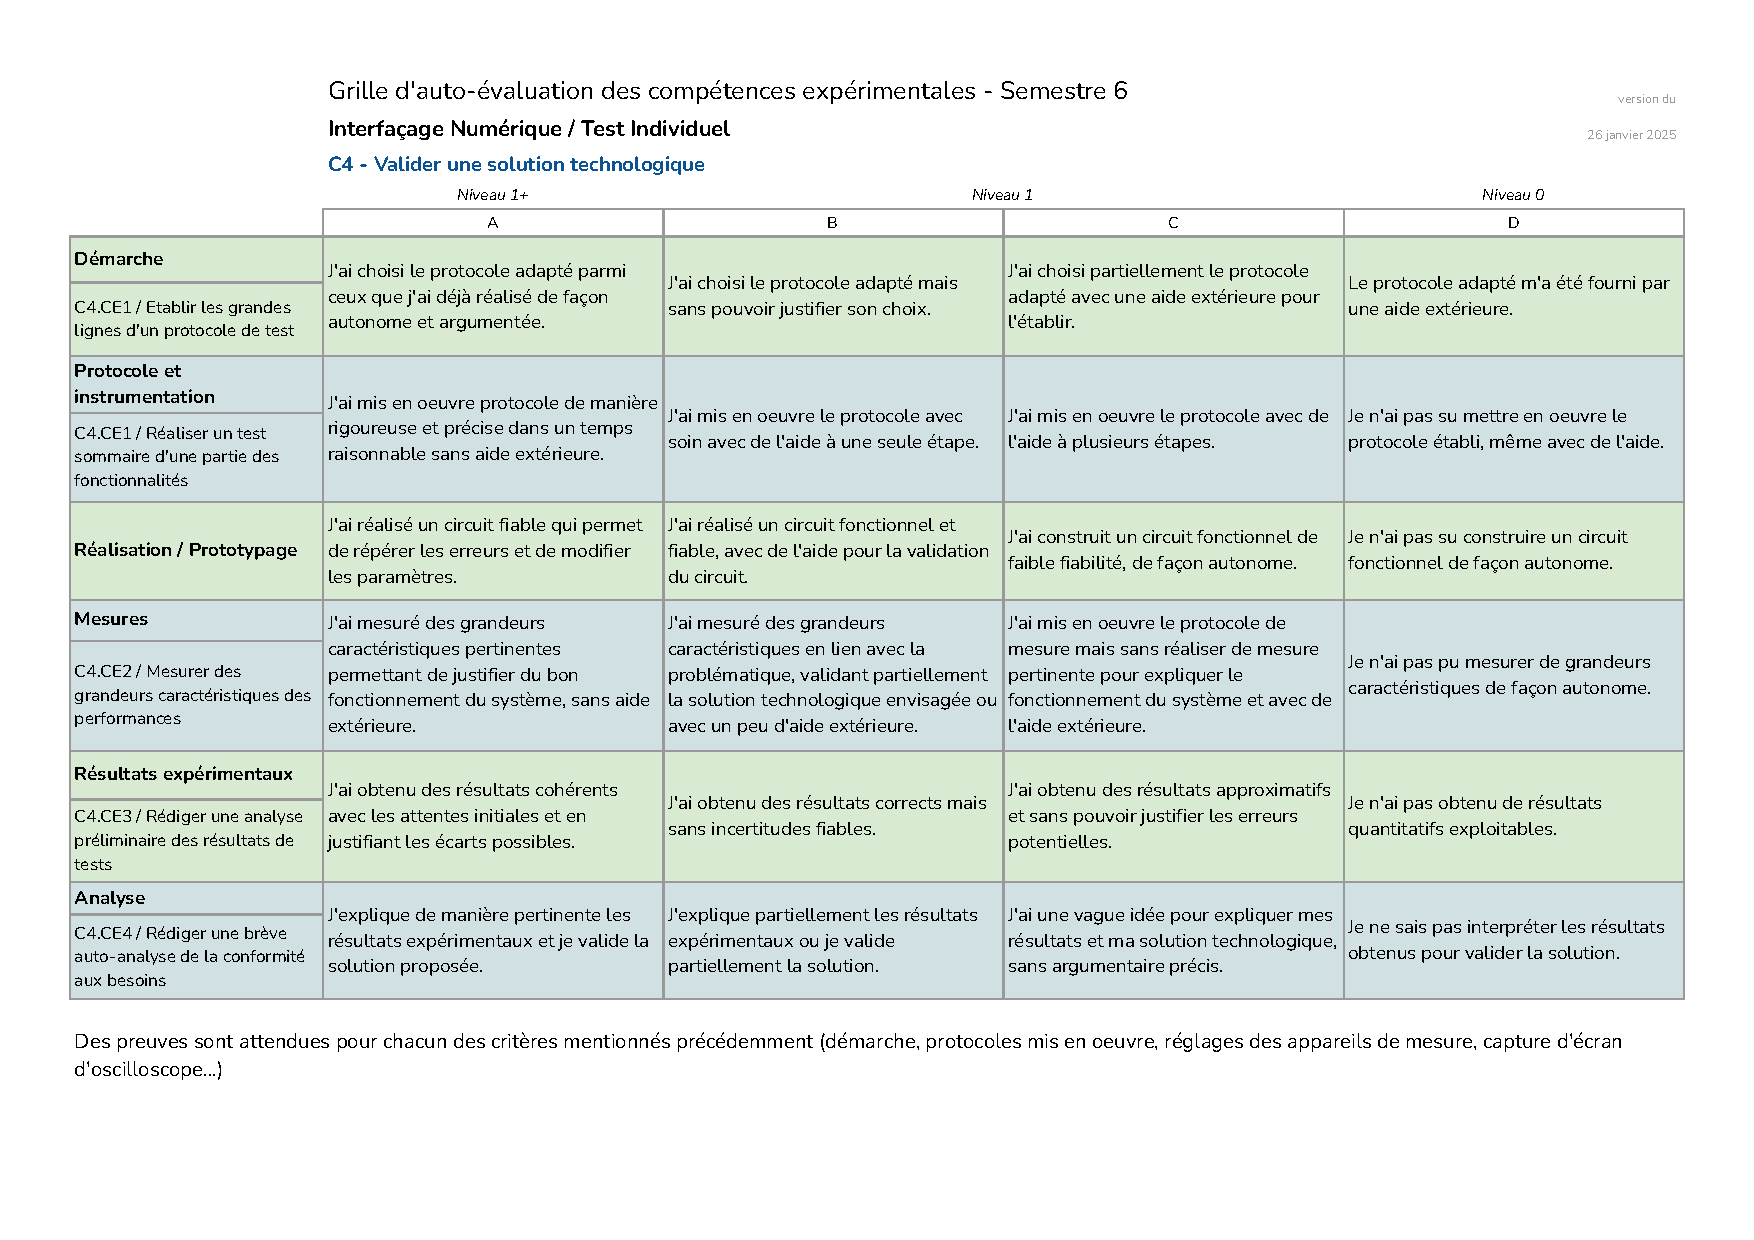
\includepdf[pages=-,landscape=true]{../S6_IntNum_2025_AutoEval_Indiv.pdf}	



\end{document}